\documentclass[12pt,a4paper]{article}
\usepackage[utf8]{inputenc}
\usepackage[english]{babel}
\usepackage[margin=1in]{geometry}
\usepackage{graphicx}
\usepackage{tikz}
\usepackage{listings}
\usepackage{booktabs}
\usepackage{float}
\usepackage{xcolor}

\usetikzlibrary{shapes,arrows,positioning}

\definecolor{codeblue}{RGB}{0,102,204}
\definecolor{codegray}{RGB}{128,128,128}
\definecolor{backcolour}{RGB}{248,248,248}

\lstset{
    basicstyle=\footnotesize\ttfamily,
    backgroundcolor=\color{backcolour},
    commentstyle=\color{codegray},
    keywordstyle=\color{codeblue},
    frame=single,
    breaklines=true,
    showstringspaces=false,
    tabsize=2
}

\title{\textbf{Air Cargo Booking \& Tracking System}\\
       \large Full-Stack Web Application Project}
\author{Keshav Laddha}
\date{\today}

\begin{document}

\maketitle

\begin{abstract}
This document presents the design and implementation of a comprehensive Air Cargo Booking and Tracking System developed as a modern full-stack web application. The system demonstrates proficiency in contemporary web technologies including React with TypeScript, Node.js with Express, and SQLite database management, implementing industry-standard patterns for authentication, state management, and API design.
\end{abstract}

\tableofcontents
\newpage

\section{Introduction}

The Air Cargo Booking and Tracking System is a comprehensive web application designed to streamline cargo booking processes and provide real-time tracking capabilities for logistics operations. This project showcases modern full-stack development practices and demonstrates technical competency in building production-ready applications.

\subsection{Project Objectives}
\begin{itemize}
    \item Develop a secure user authentication system with JWT tokens
    \item Implement intelligent flight route searching and booking workflows
    \item Create real-time cargo tracking with comprehensive status management
    \item Build responsive user interfaces with professional design patterns
    \item Design scalable API architecture following RESTful principles
\end{itemize}

\subsection{Technology Stack}
\begin{table}[H]
\centering
\begin{tabular}{@{}ll@{}}
\toprule
\textbf{Component} & \textbf{Technology} \\
\midrule
Frontend Framework & React 19.1.1 with TypeScript \\
UI Library & Material-UI (MUI) 6.5.0 \\
State Management & Redux Toolkit with RTK Query \\
Routing & React Router v7.8.2 \\
Build Tool & Vite 7.1.2 \\
Backend Runtime & Node.js with TypeScript \\
Web Framework & Express.js 4.18.2 \\
Database & SQLite 3 with custom ORM \\
Authentication & JWT with bcrypt hashing \\
Validation & Joi schema validation \\
Security & Helmet.js, CORS configuration \\
\bottomrule
\end{tabular}
\caption{Technology Stack Overview}
\end{table}

\section{System Architecture}

\subsection{High-Level Architecture}
The system implements a modern 3-tier architecture with clear separation of concerns:

\begin{figure}[H]
\centering
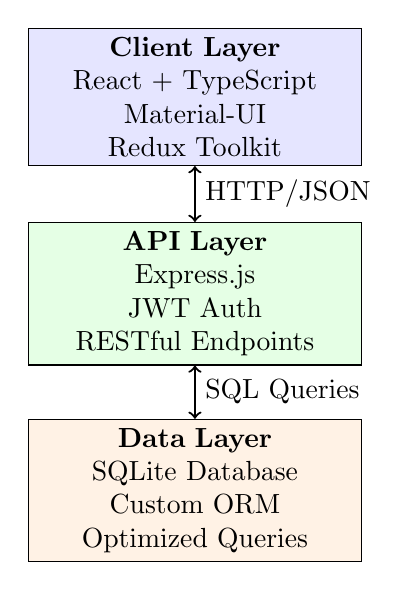
\begin{tikzpicture}[node distance=2.5cm]
    \node (client) [rectangle, draw, text width=4cm, text centered, fill=blue!10] 
        {\textbf{Client Layer}\\React + TypeScript\\Material-UI\\Redux Toolkit};
    \node (api) [rectangle, draw, text width=4cm, text centered, below of=client, fill=green!10] 
        {\textbf{API Layer}\\Express.js\\JWT Auth\\RESTful Endpoints};
    \node (data) [rectangle, draw, text width=4cm, text centered, below of=api, fill=orange!10] 
        {\textbf{Data Layer}\\SQLite Database\\Custom ORM\\Optimized Queries};
    
    \draw [<->, thick] (client) -- node[right] {HTTP/JSON} (api);
    \draw [<->, thick] (api) -- node[right] {SQL Queries} (data);
\end{tikzpicture}
\caption{System Architecture Overview}
\end{figure}

\subsection{Component Architecture}

\subsubsection{Frontend Architecture}
\begin{itemize}
    \item \textbf{Pages:} Authentication (Login/Signup), Dashboard, Search, Booking, Tracking
    \item \textbf{Components:} Reusable UI components with Material-UI integration
    \item \textbf{Store:} Redux Toolkit slices for auth, booking, and theme management
    \item \textbf{API Integration:} RTK Query for efficient data fetching and caching
\end{itemize}

\subsubsection{Backend Architecture}
\begin{itemize}
    \item \textbf{Controllers:} AuthController, BookingsController, RoutesController
    \item \textbf{Services:} Business logic layer (AuthService, RouteService, TimelineService)
    \item \textbf{Models:} Data access layer (User, Booking models)
    \item \textbf{Middleware:} Authentication, validation, error handling
\end{itemize}

\section{Database Design}

\subsection{Schema Overview}
The database schema is designed for optimal performance with proper indexing and referential integrity:

\begin{table}[H]
\centering
\small
\begin{tabular}{@{}lll@{}}
\toprule
\textbf{Table} & \textbf{Purpose} & \textbf{Key Fields} \\
\midrule
users & User authentication & id, username, email, password\_hash \\
airlines & Airline information & id, code, name \\
flights & Flight schedules & id, flight\_number, origin, destination \\
bookings & Cargo bookings & id, ref\_id, user\_id, status, flight\_ids \\
timeline\_events & Tracking history & id, booking\_id, event\_type, location \\
booking\_counters & Reference generation & date\_key, counter \\
\bottomrule
\end{tabular}
\caption{Database Schema Tables}
\end{table}

\subsection{Key Features}
\begin{itemize}
    \item Foreign key constraints with CASCADE operations
    \item Optimized indexes for frequent query patterns
    \item JSON fields for flexible flight sequence storage
    \item Check constraints for data integrity
    \item Automated reference ID generation system
\end{itemize}

\section{API Design}

\subsection{RESTful Endpoints}
\begin{table}[H]
\centering
\footnotesize
\begin{tabular}{@{}llll@{}}
\toprule
\textbf{Method} & \textbf{Endpoint} & \textbf{Purpose} & \textbf{Auth} \\
\midrule
POST & /api/v1/auth/signup & User registration & No \\
POST & /api/v1/auth/login & User authentication & No \\
GET & /api/v1/auth/profile & Get user profile & Yes \\
GET & /api/v1/auth/validate & Validate JWT token & No \\
\midrule
GET & /api/v1/routes & Search flight routes & No \\
POST & /api/v1/routes/validate & Validate flight sequence & No \\
\midrule
POST & /api/v1/bookings & Create new booking & Yes \\
GET & /api/v1/bookings/my-bookings & Get user bookings & Yes \\
GET & /api/v1/bookings/:ref/history & Get booking timeline & No \\
PUT & /api/v1/bookings/:ref/depart & Update to departed & Yes \\
PUT & /api/v1/bookings/:ref/arrive & Update to arrived & Yes \\
PUT & /api/v1/bookings/:ref/cancel & Cancel booking & Yes \\
\bottomrule
\end{tabular}
\caption{API Endpoints Overview}
\end{table}

\subsection{Response Format}
All API responses follow a consistent JSON structure:

\begin{lstlisting}[caption=Standard API Response Format]
{
  "message": "Operation successful",
  "data": {
    // Response payload
  },
  "error": "Error description (if applicable)"
}
\end{lstlisting}

\section{Implementation Highlights}

\subsection{Authentication System}
Secure JWT-based authentication with bcrypt password hashing:

\begin{lstlisting}[caption=Authentication Implementation]
// AuthService.ts - User authentication
static async authenticateUser(email: string, password: string) {
  const user = await User.findByEmail(email);
  
  if (user && bcrypt.compareSync(password, user.password_hash)) {
    const token = jwt.sign(
      { userId: user.id, email: user.email },
      JWT_SECRET,
      { expiresIn: '24h' }
    );
    return { user, token };
  }
  
  return null;
}
\end{lstlisting}

\subsection{State Management}
Redux Toolkit implementation with persistence:

\begin{lstlisting}[caption=Redux Store Configuration]
// store/index.ts
export const store = configureStore({
  reducer: {
    auth: authSlice,
    booking: bookingSlice,
    theme: themeSlice,
    api: apiSlice.reducer,
  },
  middleware: (getDefaultMiddleware) =>
    getDefaultMiddleware({
      serializableCheck: {
        ignoredActions: ['persist/PERSIST', 'persist/REHYDRATE'],
      },
    }).concat(apiSlice.middleware),
});
\end{lstlisting}

\subsection{Database Operations}
Custom ORM with transaction support:

\begin{lstlisting}[caption=Database Transaction Example]
// Booking creation with timeline event
try {
  await database.beginTransaction();
  
  const booking = await Booking.create(bookingData);
  
  await TimelineEvent.create({
    booking_id: booking.id,
    event_type: 'CREATED',
    notes: 'Booking created successfully'
  });
  
  await database.commit();
  return booking;
} catch (error) {
  await database.rollback();
  throw error;
}
\end{lstlisting}

\section{Security Implementation}

\subsection{Security Measures}
\begin{itemize}
    \item JWT tokens with 24-hour expiration
    \item bcrypt password hashing with salt rounds
    \item Helmet.js for HTTP header security
    \item CORS configuration for cross-origin requests
    \item Input validation using Joi schemas
    \item SQL injection prevention through parameterized queries
\end{itemize}

\subsection{Error Handling}
Comprehensive error handling with proper HTTP status codes:

\begin{lstlisting}[caption=Global Error Handler]
// middleware/errorHandler.ts
export const errorHandler = (err: any, req: Request, res: Response, next: NextFunction) => {
  // Joi validation errors
  if (err.isJoi) {
    return res.status(400).json({
      error: 'VALIDATION_ERROR',
      message: err.details[0].message
    });
  }
  
  // Database constraint errors
  if (err.code === 'SQLITE_CONSTRAINT') {
    return res.status(409).json({
      error: 'CONSTRAINT_VIOLATION',
      message: 'Data integrity constraint violated'
    });
  }
  
  // Default server error
  res.status(500).json({
    error: 'INTERNAL_SERVER_ERROR',
    message: 'An unexpected error occurred'
  });
};
\end{lstlisting}

\section{Frontend Implementation}

\subsection{Component Structure}
Modular React components with TypeScript:

\begin{itemize}
    \item \textbf{Layout Components:} Main layout with navigation and theme switching
    \item \textbf{Page Components:} Login, Signup, Dashboard, Search, Booking, Tracking
    \item \textbf{Common Components:} LoadingSpinner, forms, and utility components
    \item \textbf{Protected Routes:} Route guards based on authentication state
\end{itemize}

\subsection{Material-UI Integration}
\begin{lstlisting}[caption=Theme Configuration]
// theme/index.ts
export const lightTheme = createTheme({
  palette: {
    mode: 'light',
    primary: {
      main: '#1976d2',
    },
    secondary: {
      main: '#dc004e',
    },
  },
  typography: {
    fontFamily: 'Roboto, Arial, sans-serif',
  },
});
\end{lstlisting}

\section{Performance Optimizations}

\subsection{Database Optimizations}
\begin{itemize}
    \item Strategic indexing on frequently queried columns
    \item Composite indexes for complex query patterns
    \item Connection pooling and transaction management
    \item Query optimization for route searching
\end{itemize}

\subsection{Frontend Optimizations}
\begin{itemize}
    \item Redux state persistence for improved UX
    \item RTK Query for efficient data caching
    \item Lazy loading of route components
    \item Material-UI theme optimization
\end{itemize}

\section{Testing \& Quality Assurance}

\subsection{Development Practices}
\begin{itemize}
    \item TypeScript for compile-time type checking
    \item ESLint for code quality enforcement
    \item Comprehensive API testing with Postman
    \item Manual testing of all user workflows
    \item Error boundary implementation
\end{itemize}

\subsection{Deployment Readiness}
\begin{itemize}
    \item Environment configuration management
    \item Production build optimization
    \item Graceful shutdown handling
    \item Health check endpoints
    \item Docker containerization support
\end{itemize}

\section{Project Outcomes}

\subsection{Technical Achievements}
\begin{itemize}
    \item \textbf{Full-Stack Proficiency:} Complete application from database to UI
    \item \textbf{Modern Architecture:} Industry-standard patterns and practices
    \item \textbf{Security Implementation:} Comprehensive security measures
    \item \textbf{Performance Optimization:} Efficient queries and state management
    \item \textbf{Code Quality:} TypeScript, ESLint, and modular architecture
\end{itemize}

\subsection{Professional Skills Demonstrated}
\begin{itemize}
    \item Problem-solving through systematic design approach
    \item API design following RESTful principles
    \item Database modeling and optimization
    \item User experience design with responsive interfaces
    \item Project planning and documentation
\end{itemize}

\section{Future Enhancements}

\subsection{Scalability Improvements}
\begin{itemize}
    \item Migration to PostgreSQL for production scaling
    \item Redis caching layer for improved performance
    \item Microservices architecture for large-scale deployment
    \item Container orchestration with Kubernetes
\end{itemize}

\subsection{Feature Extensions}
\begin{itemize}
    \item Real-time notifications with WebSocket integration
    \item Payment processing with Stripe integration
    \item Advanced analytics and reporting dashboard
    \item Mobile application with React Native
    \item Integration with external airline APIs
\end{itemize}

\section{Conclusion}

The Air Cargo Booking and Tracking System successfully demonstrates comprehensive full-stack development capabilities using modern web technologies. The project showcases:

\begin{itemize}
    \item \textbf{Technical Expertise:} Proficiency in React, Node.js, TypeScript, and database design
    \item \textbf{Industry Standards:} Implementation of security best practices and architectural patterns
    \item \textbf{Professional Quality:} Production-ready code with comprehensive error handling
    \item \textbf{Scalable Design:} Architecture capable of handling real-world requirements
\end{itemize}

This project represents a complete software development lifecycle from requirements analysis through implementation and testing, demonstrating readiness for professional software development roles.

\vspace{1cm}
\hrule
\begin{center}
\textit{Air Cargo Booking \& Tracking System}\\
\textbf{Full-Stack Web Application}\\
Developed by Keshav Laddha - \today
\end{center}

\end{document}